\section{VLSI implementation}

Lo scopo di questa sezione è quello di presentare l'implementazione del filtro IIR progettato, che nella fattispecie è un filtro IIR con precisione di 10 bit e ordine pari a 1. In \autoref{fig:filtro_generic} {\LARGE correggere} è mostrata l'interfaccia del filtro dove il parallelismo $n_b$ è fissato a 10 ed essendo l'ordine del filtro pari a 1, i coefficienti necessari sono $a_0, a_1, b_0, b_1$. 

\begin{figure}[h]
	\center
	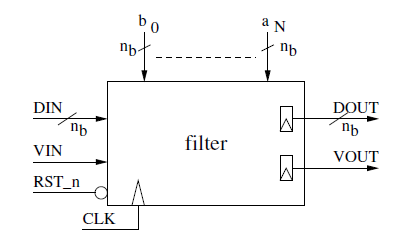
\includegraphics[width=0.4\textwidth]{filtro_generic.png}
	\caption{Filter pinout}
	\label{fig:filtro_generic}
\end{figure}


\subsection{VHDL model}
In ingresso e in uscita al filtro sono posti dei registri per sincronizzare i dati con il clock e due segnali di validazione per i dati, $VIN$ and $VOUT$. In \autoref{fig:IIR_1} è mostrata l'architettura del filtro, dove i registri sono stati trascurati, la forma utilizzata è la direct form II. I dati in ingresso campionati entrano dalla porta $x[n]$, vengono elaborati e i risultati fuoriescono dalla porta $y[n]$. Il parallelismo interno della macchina è diverso da quello esterno, per evitare la possibilità di avere overflow con qualsiasi combinazione di dati in ingresso quando viene effettuata la somma, la precisione è stata estesa a 12 bit effettuando un'estensione del segno a tutti i segnali in ingresso. La moltiplicazione invece non ha problemi di parallelismo perché si riesce ad avere una precisione sufficiente troncando i bit meno significativi ad ogni moltiplicazione e avendo quindi stesso parallelismo tra dati in ingresso e in uscita. Il registro interno alla macchina ha un segnale di enable che viene gestito dal segnale di validazione del dato in ingresso in modo che quando si ricevono dati non validi, esso non campiona mantenendo il dato in uscita corretto.

\begin{figure}[h]
	\center
	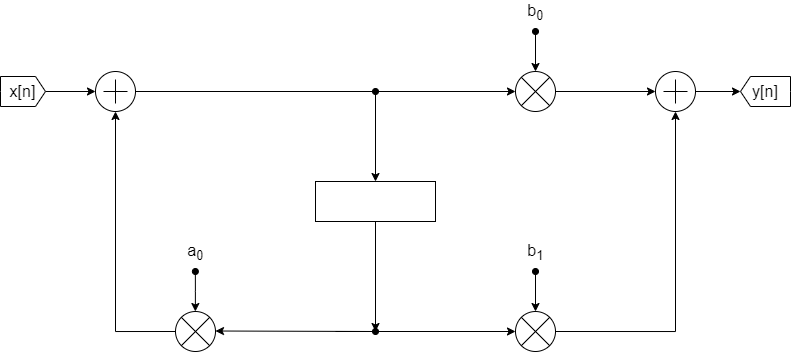
\includegraphics[width=0.8\textwidth]{iir_1.png}
	\caption{IIR filter architecture}
	\label{fig:IIR_1}
\end{figure}

\subsection{Simulation}

\subsection{Logic Synthesis}

\subsection{Place \& Route}